% Please use the skeleton file you have received in the
% invitation-to-submit email, where your data are already
% filled in. Otherwise please make sure you insert your
% data according to the instructions in PoSauthmanual.pdf
\documentclass{PoS}

\usepackage{wrapfig}
\title{Recent Developments of the fastNLO Toolkit}

\ShortTitle{Recent Developments of the fastNLO Toolkit}

\author{Daniel Britzger\\
        DESY\\
        E-mail: \email{daniel.britzger@desy.de}}
\author{Klaus Rabbertz, Georg Sieber\\
        Karlsruhe Institute of Technology\\
        E-mail: \email{klaus.rabbertz@cern.ch}, \email{georg.sieber@cern.ch}}
\author{\speaker{Fred Stober}\\
        Karlsruhe Institute of Technology (at the time of the presentation), University of Hamburg\\
        E-mail: \email{stober@cern.ch}}
\author{Markus Wobisch\\
        Louisiana Tech University\\
        E-mail: \email{wobisch@fnal.gov}}

\abstract{
The precise calculation of hadron-hadron collisions at higher orders of
perturbative QCD requires a large amount of processing power.
In addition, thorough analyses require that these calculations are
repeated many times for different parameters.
The fastNLO toolkit can be interfaced with next-to-leading order (NLO)
and next-to-next-to-leading order (NNLO) Monte-Carlo programs to make
these computations more efficient.
Using multi-dimensional interpolation techniques, coefficient tables are
produced that allow to quickly evaluate the cross section for
different PDFs, values of $\alpha_s$ and scale choices.

These proceedings focuses on recent developments of the fastNLO framework, in
particular on the increased flexibility with respect to scale variations
and the new generators that are already interfaced.
As an example, the flexibility of fastNLO is shown using a measurement
of the strong coupling constant, where the $\alpha_s$ evolution is modified
to refine the fitting procedure.}

\FullConference{XXIII International Workshop on Deep-Inelastic Scattering\\
		27 April - May 1 2015\\
		Dallas, Texas}


\begin{document}

\section{Introduction}

Very accurate theoretical predictions are crucial for modern
precision measurements in high energy physics.
However, such theory calculations of observables at higher orders
of perturbative QCD can be very challenging and often take a very long
time. In addition, it is often necessary to repeat these complex
calculations for a large set of different parameters. Typical examples for such variations are:

\begin{itemize}
\item The comparison of precision measurements with theory are usually
  performed with several sets of parton distribution functions (PDFs),
  that are provided by different PDF fitting groups. %(PDF4LHC)\cite{Rojo:2015acz}.
\item The uncertainty assessment of a single PDF set can require
  the evaluation of the theory predictions for a number of different
  PDF uncertainty eigenvectors or PDF replicas. The NNPDF~\cite{Ball:2014uwa} uncertainty
  prescription for example requires to evaluate the sample variance on a set of
  $100$ to $1000$ different PDF replicas.
\item For the estimation of the effect of missing higher orders in theory
  predictions, the calculations are conventionally repeated for different
  choices of the renormalization and/or factorization scale. For processes
  involving multiple scales it is often necessary to also
  investigate these scale variations as a function of different observables of
  the processes.
\item The determination of theory parameters from measurements, like
  the value of the strong coupling constant or constraining PDFs,
  requires the evaluation of theory predictions for different values
  of these parameters.
  The fit procedure for PDFs involves the recalculation
  of theory predictions for a large number of different observables due to
  the parameter changes in the underlying PDFs in each step of the fitting procedure.
  FastNLO is used by various PDF fitting groups,
  like ABM~\cite{Alekhin:2013nda}, CTEQ-JLAB~\cite{Owens:2012bv},
  CTEQ-TEA~\cite{Dulat:2015mca}, HERAPDF~\cite{Abramowicz:2015mha},
  MMHT~\cite{Harland-Lang:2014zoa}, or NNPDF~\cite{Ball:2014uwa}.
\end{itemize}

In particular for observables like Drell-Yan and jet cross sections at
hadron-hadron colliders, the evaluation of these variations using only
the next-to-leading order (NLO) or next-to-next-to-leading order (NNLO)
code can quickly become impractical.
fastNLO~\cite{Britzger:2012bs,Wobisch:2011ij,Kluge:2006xs} was developed
to substantially reduce the amount of processing power that is needed to
investigate different variations of predictions for observables in
NLO or even higher-order.
%The fastNLO package is uses NLO or NNLO Monte-Carlo programs to generate
%interpolation tables. These tables enable the very fast computation of these observables for
%different PDFs, values of $\alpha_s(M_\mathrm{Z})$, and also give the opportunity to
%change the functional form of the scales.

\subsection{fastNLO fundamentals}

Perturbative QCD predictions for observables in hadron-induced
processes depend on the strong coupling constant $\alpha_s$ and on the
PDFs of the hadron(s). Any cross section in lepton-hadron or
hadron-hadron collisions can expressed in terms of the
strong coupling constant to the power of $n$, $\alpha_s^n$, the
perturbative coefficients $c_{i,n}$ for the partonic subprocess $i$,
and the corresponding linear combination of PDFs from the one or two
hadrons $f_i$, which is a function of the fractional hadron momenta
$x_1$, $x_2$ carried by the respective partons.
The equation describing hadron-hadron cross sections with subprocess $i=(a,b)$
for the interaction of parton $a$, $b$ in particular is given by:
\begin{equation}\label{eq:CrossSection}
  \sigma_{pp\rightarrow\mathrm{X}}(\mu_r,\mu_f) =
  \sum\limits_{a,b,n}\int\limits_0^1dx_1\int\limits_0^1dx_2
    \alpha_s^n(\mu_r) c_{(a,b),n} f_{1,a}(x_1,\mu_f) f_{2,b}(x_2,\mu_f)
\end{equation}

%Due to the necessary Monte-Carlo phase-space integration, the calculation
%of this cross section can take a long time to reach a reasonably small
%statistical uncertainty.
The fundamental concept behind fastNLO is to isolate the perturbative
coefficients $c_{i,n}$ from the PDFs and the $\alpha_s$ factors and thereby
convert this integration into a sum~\cite{Pascaud:1994vx,Wobisch:00}.
This discretization introduces a set of eigenfunctions $E_k(x)$
(with $\sum_k E_k(x) \equiv 1$) around a defined number of $x$-values.
The PDFs $f_p(x_p)$ in equation~\ref{eq:CrossSection} can then be replaced
by $f_p \simeq \sum_k f_p(x_k) E_k(x)$ and moved in front of the integral.
The remaining integration over $x$ to compute the cross section is
turned into a sum over the $n$ perturbative orders, $i$ parton flavors,
and all the $x$-nodes.

The perturbative coefficients $c_{i,n}$ can be further decomposed to describe
the dependence on the renormalization and factorization scales $\mu_r, \mu_f$
at NLO with $c_{i,n}^0$,$c_{i,n}^r$,$c_{i,n}^f$ and NNLO with
$c_{i,n}^rr$,$c_{i,n}^rf$,$c_{i,n}^ff$:
\begin{eqnarray}\label{eq:ScaleIndependentWeights}
  c_{i,n}(\mu_r,\mu_f) &=& c_{i,n}^0 + \log(\mu_r)c_{i,n}^r +  \log(\mu_f) c_{i,n}^f \nonumber \\
     &&+ \log(\mu_r^2)c_{i,n}^rr + \log(\mu_f^2) c_{i,n}^ff + \log(\mu_r^2)\log(\mu_f^2) c_{i,n}^rf
\end{eqnarray}

For the determination of the renormalization scale variations, fastNLO allows
to either use the RGE in conjunction with the leading-order matrix element,
or directly store the scale-independent weights from equation \ref{eq:ScaleIndependentWeights}.
Variations of the factorization scale can be done by either storing the
coefficients for a fixed set of factorization scales, by using the LO DGLAP
splitting functions from HOPPET~\cite{Salam:2008qg}, or by simply storing
the scale-independent weights as above.

The perturbative coefficients only need to be calculated once with
very high statistical precision, with the weights describing these
coefficients being stored in an interpolation table.
These tables can be enriched with additional additive or multiplicative
contributions to the cross sections.

\begin{wrapfigure}{r}{0.5\textwidth}
 \centering
  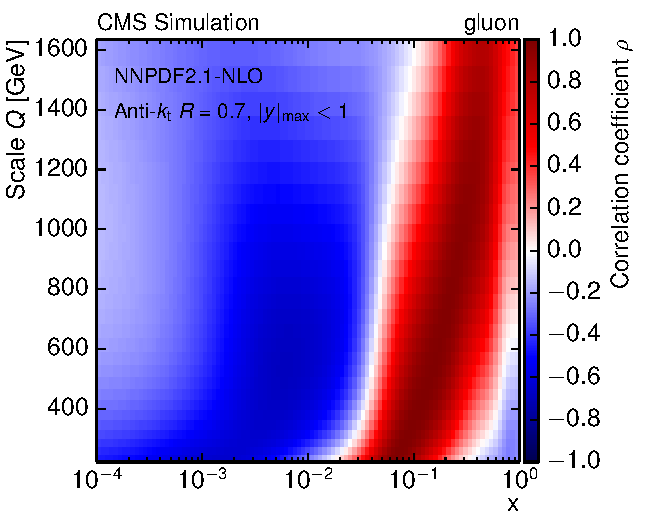
\includegraphics[width=0.49\textwidth]{05_correlation_g_0_1}
  \caption{Correlations between the gluon PDF and the three-jet production cross section
  as a function of x and the scale of the process\cite{CMS:2014mna}.}
  \label{Fig:correlations}
\end{wrapfigure}

It is also possible to include measurements and (un-)correlated uncertainties in a single table.
When processing these tables, the summation of weights can be adapted
to different PDFs, values of $\alpha_s$ or scale choices. This allows to quickly perform
all needed variations in a fraction of the time needed to do the full
calculation.

An example for an application of these techniques is shown in figure~\ref{Fig:correlations},
which presents the correlation between the gluon PDF and the three-jet production
cross section in proton-proton collision events.
In order to calculate these correlations, three-jet production cross sections
were evaluated for all of the 100 PDF replicas of the NNPDF 2.1~\cite{Ball:2011uy}
PDF set within seconds. Since fastNLO provides information about the average
scale that is used in each observable bin, the correlation
between the cross section and the gluon PDF could be shown as a function
of x and the scale of the process.

\newpage
\section{Recent developments}

\begin{wrapfigure}{r}{0.5\textwidth}
  \centering
  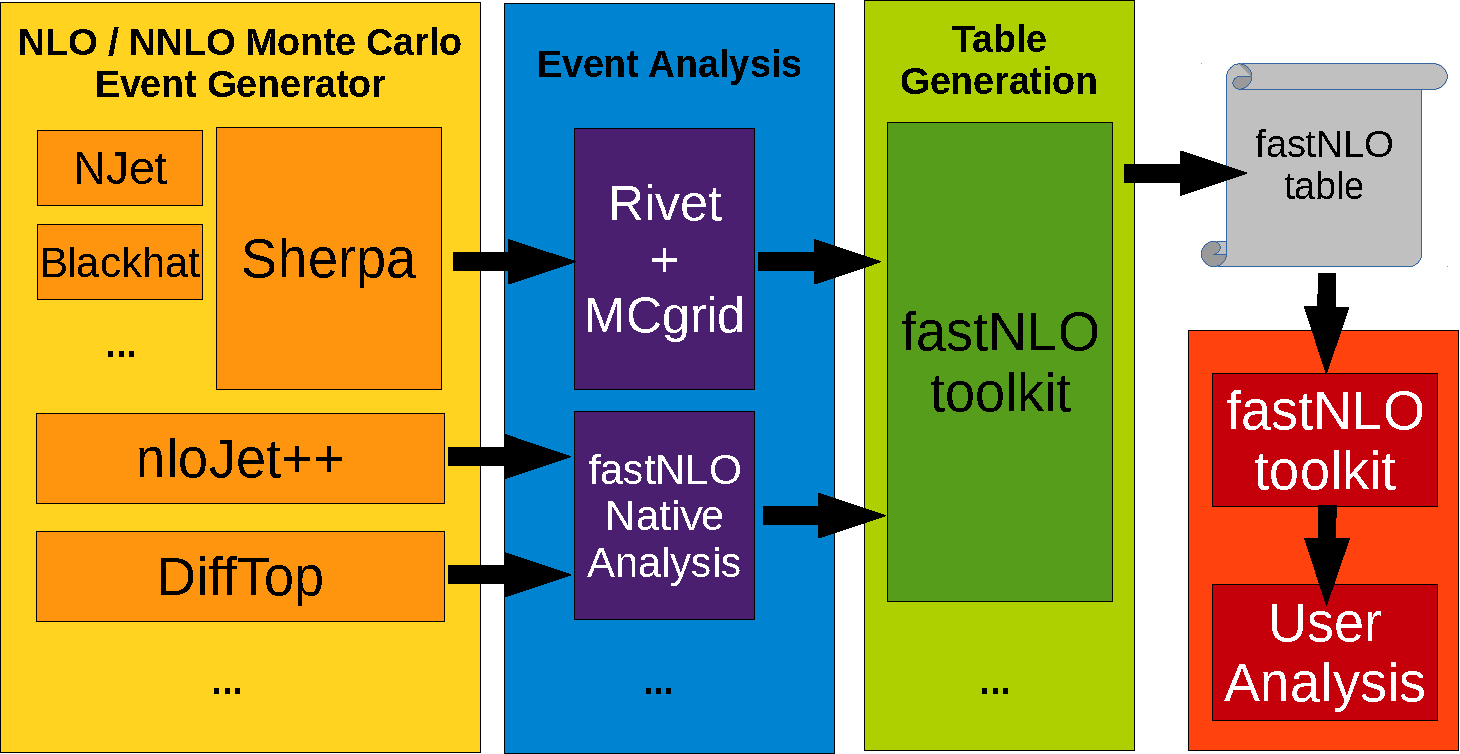
\includegraphics[width=0.49\textwidth]{interface-crop}
  \caption{Overview of the fastNLO processing workflow. Several
    NLO and NNLO generators are directly or indirectly (via \texttt{MCgrid}+\texttt{RIVET})
    interfaced to fastNLO and can be used to create interpolation tables.
    These tables can be used to quickly evaluate theory predictions
    for different PDFs, $\alpha_s$ or scale choices.}
  \label{Fig:interface}
\end{wrapfigure}

While fastNLO was already directly interfaced to some important (N)NLO generators
like \texttt{NLOJet++}~\cite{Nagy:1998bb,Nagy:2001xb,Nagy:2003tz} or DiffTop~\cite{Guzzi:2014wia},
the recently developed interface to \texttt{MCgrid}~\cite{DelDebbio:2013kxa}
enables access to Monte Carlo generators like \texttt{Sherpa}\cite{Gleisberg:2008ta}
and the analysis code contained in \texttt{RIVET}~\cite{Buckley:2010ar}.

The new fastNLO toolkit has a clean interface to implement interfaces
to additional (N)NLO Monte-Carlo in order to create tables.
It also provides users with simple to use interfaces in C++, Fortran
and Python to read tables and calculate cross sections using existing
PDFs and $\alpha_s$ evolution codes as provided by
\texttt{LHAPDF 5/6}~\cite{Buckley:2014ana,Bourilkov:2006cj} for example.
For advanced users it is also possible to provide own PDFs and
$\alpha_s$ evolution codes in C++ or Fortran that can be used in the table evaluation.

\section{fastNLO in action}

\begin{wrapfigure}{r}{0.5\textwidth}
  \centering
  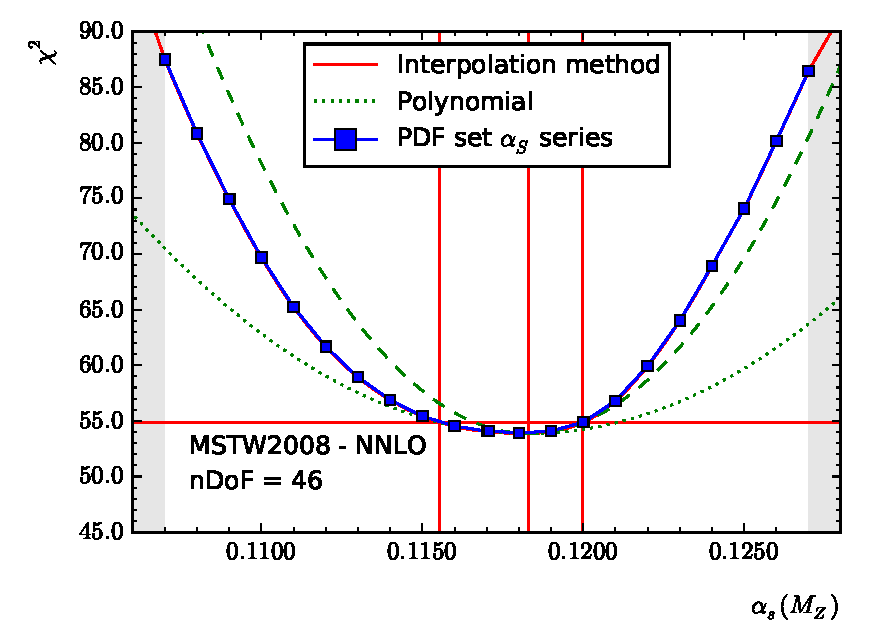
\includegraphics[width=0.49\textwidth]{chi2cmp}
  \caption{Comparison between the commonly used $\alpha_s$ fit method (green)
  and the refined method (red). The $\chi^2$ is calculated from the measurement
  of the three-jet production cross section\cite{CMS:2014mna} and theory predictions (\texttt{NLOJet++} with MRST2008 PDF\cite{Martin:2009iq}).
  }
  \label{Fig:chi2}
\end{wrapfigure}
The flexibility of fastNLO with respect to the $\alpha_s$ evolution
that is employed during the table evaluation allows to refine the
fit procedure for $\alpha_s(M_\mathrm{Z})$ as it is used by
experiments\cite{Affolder:2001hn,Chatrchyan:2013txa}
.%with observables that are sensitive to $\alpha_s$.

Since global PDF fits are only provided for a limited set of
$\alpha_s(M_\mathrm{Z})$ values, the common procedure calculates the
$\chi^2$ between data and the theory predictions
that are given by the $\alpha_s$ series.
The fit result is then derived from a parametrisation (usually
a simple polynomial of order 2) of the $\chi^2$ curve.

The refined method replaces the
$\alpha_s$ evolution code in fastNLO that is provided by \texttt{LHAPDF} with
another $\alpha_s$ evolution code\cite{GRV} that allows to freely
choose the value of $\alpha_s(M_\mathrm{Z})$. This allows to calculate
arbitrary values of $\chi^2(\alpha_s(M_\mathrm{Z}))$ without resorting
to parametrisations and enables the application of common
minimization libraries to derive the central fit result and the
uncertainties.

As shown in figure~\ref{Fig:chi2}, the refined method directly provides
a straightforward description of the uncertainties without any ambiguities
introduced by choosing some parametrisation.

\subsection{Mathematical description of the refined method}

Mathematically, this replacement can be described with the following set of equations.
Any observable $O$ that can be calculated by fastNLO can be expressed as:
\begin{eqnarray}
O = O(\mathrm{PDF}^i(
	\alpha_s^\mathrm{PDF,i}(\alpha_s^\mathrm{PDF,i}(M_\mathrm{Z,i}), M_\mathrm{Z,i}, Q)),
	\alpha_s^\mathrm{fastNLO}(\alpha_s^\mathrm{fastNLO}(M_\mathrm{Z}), M_\mathrm{Z}, Q))
\end{eqnarray}
$\mathrm{PDF}^i$ is a PDF member $i$ that is provided by a PDF fitter group together with
a certain $\alpha_s^\mathrm{PDF,i}$ evolution for a given $\alpha_s^\mathrm{PDF,i}(M_\mathrm{Z,i})$.
By default, fastNLO evaluates the observable with:
\begin{eqnarray}
\alpha_s^\mathrm{fastNLO}(\alpha_s^\mathrm{fastNLO}(M_\mathrm{Z}), M_\mathrm{Z}, Q) = 
\alpha_s^\mathrm{PDF,i}(\alpha_s^\mathrm{PDF,i}(M_\mathrm{Z,i}), M_\mathrm{Z,i}, Q)
\end{eqnarray}
However for the presented method $\alpha_s^\mathrm{fastNLO}(\alpha_s^\mathrm{fastNLO}(M_\mathrm{Z}), M_\mathrm{Z}, Q)$
can be any $\alpha_s$ evolution code, where $\alpha_s^\mathrm{fastNLO}(M_\mathrm{Z})$ can be choosen freely.
In order to guarantee perfect agreement for the observable when calculated with
the exact calculation at $\alpha_{s}^\mathrm{fastNLO}(M_\mathrm{Z}) = \alpha_s^\mathrm{PDF,i}(M_\mathrm{Z,i})$,
a correction factor $k_i$ is defined by:
\begin{eqnarray}
k_i = \frac{
	O(\mathrm{PDF}^i(
		\alpha_s^\mathrm{PDF,i}(\alpha_s^\mathrm{PDF,i}(M_\mathrm{Z,i}), M_\mathrm{Z,i}, Q)),
		\alpha_s^\mathrm{PDF,i}(\alpha_s^\mathrm{PDF,i}(M_\mathrm{Z,i}), M_\mathrm{Z,i}, Q))
	}{
	O(\mathrm{PDF}^i(
		\alpha_s^\mathrm{PDF,i}(\alpha_s^\mathrm{PDF,i}(M_\mathrm{Z,i}), M_\mathrm{Z,i}, Q)),
		\alpha_s^\mathrm{fastNLO}(\alpha_s^\mathrm{PDF,i}(M_\mathrm{Z,i}), M_\mathrm{Z}, Q))
	}
\end{eqnarray}
This correction factor is usually very small and on the permille level.
The observable $\mathcal{O}_i(\alpha_s(M_\mathrm{Z}))$ represents an extrapolation of $O$
calculated for a PDF member $i$ with associated $\alpha_s^\mathrm{PDF,i}(M_\mathrm{Z,i})$
to arbitary values of $\alpha_s(M_\mathrm{Z})$ and takes the form:
\begin{eqnarray}
\mathcal{O}_i(\alpha_s(M_\mathrm{Z})) = k_i \cdot O(\mathrm{PDF}^a(
		\alpha_s^\mathrm{PDF,i}(\alpha_s^\mathrm{PDF,i}(M_\mathrm{Z,i}), M_\mathrm{Z,i}, Q)),
		\alpha_s^\mathrm{fastNLO}(\alpha_s(M_\mathrm{Z}), M_\mathrm{Z}, Q))
\end{eqnarray}

The refined method presented above calculates $\chi^2(\alpha_s(M_\mathrm{Z}))$ values outside the
$\alpha_s(M_\mathrm{Z})$ range provided by the PDF fitter groups from
$\mathcal{O}_i(\alpha_s(M_\mathrm{Z}))$, where $i$ is the PDF member with the smallest or largest value of
$\alpha_s^\mathrm{PDF,i}(M_\mathrm{Z,i})$.

In order to calculate $\mathcal{O}(\alpha_s(M_\mathrm{Z}))$ for some arbitary $\alpha_s(M_\mathrm{Z})$ within the
range provided by the PDF fitter groups, the PDF members $a$ and $b$ are used
whose $\alpha_s^\mathrm{PDF,i}(M_\mathrm{Z,i})$ values are closest to $\alpha_s(M_\mathrm{Z})$ with:
\begin{eqnarray}
\alpha_s^\mathrm{PDF,a}(M_\mathrm{Z,a}) \leq \alpha_s(M_\mathrm{Z}) \leq \alpha_s^\mathrm{PDF,b}(M_\mathrm{Z,b})
\end{eqnarray}

The value for $\mathcal{O}(\alpha_s(M_\mathrm{Z}))$ is based on a simple linear interpolation between $\mathcal{O}_a$ and $\mathcal{O}_b$:
\begin{eqnarray}
\mathcal{O}(\alpha_s(M_\mathrm{Z})) =
\mathcal{O}_a(\alpha_s(M_\mathrm{Z})) +
\left( \mathcal{O}_b(\alpha_s(M_\mathrm{Z})) - \mathcal{O}_a(\alpha_s(M_\mathrm{Z})) \right) \cdot
	\frac{
		\alpha_s(M_\mathrm{Z}) - \alpha_s^\mathrm{PDF,a}(M_\mathrm{Z,a})
	}{
		\alpha_s^\mathrm{PDF,b}(M_\mathrm{Z,b}) - \alpha_s^\mathrm{PDF,a}(M_\mathrm{Z,a})
	}
\end{eqnarray}

The linear interpolation and the correction factors ensure a continous behaviour
of $\mathcal{O}(\alpha_s(M_\mathrm{Z}))$ for all $\alpha_s(M_\mathrm{Z})$ and
perfect agreement with the calculations from the $\alpha_s$ series provided by the PDF:
\begin{eqnarray}
\mathcal{O}(\alpha_s^\mathrm{PDF,i}(M_\mathrm{Z,i})) = O(\mathrm{PDF}^i(
		\alpha_s^\mathrm{PDF,i}(\alpha_s^\mathrm{PDF,i}(M_\mathrm{Z,i}), M_\mathrm{Z,i}, Q)),
		\alpha_s^\mathrm{PDF,i}(\alpha_s^\mathrm{PDF,i}(M_\mathrm{Z,i}), M_\mathrm{Z,i}, Q))
\end{eqnarray}
for $i = a,b$.

\newpage
\bibliographystyle{lucas_unsrt}
\bibliography{dis2015_stober}

\end{document}
